\documentclass[]{beamer}
% Class options include: notes, notesonly, handout, trans,
%                        hidesubsections, shadesubsections,
%                        inrow, blue, red, grey, brown

% Theme for beamer presentation.
\usepackage{beamerthemesplit} 
% Other themes include: beamerthemebars, beamerthemelined, 
%                       beamerthemetree, beamerthemetreebars  

\title{WIRELESS COMMUNICATION USING TV WHITE SPACE}    % Enter your title between curly braces
\author{Charles Bundala\\Wilson Chanhemo\\Said A Kombo\\ Noel Chintelele}                 % Enter your name between curly braces
\institute{University of Dodoma}      % Enter your institute name between curly braces
\date{\today}  
\linespread{1.5}                  % Enter the date or \today between curly braces

\begin{document}

% Creates title page of slide show using above information
\begin{frame}
 \titlepage
\end{frame}     % typeset with the notes or notesonly class options

\begin{frame}{\centering OUTLINE}
  \begin{itemize}
  \item OVERVIEW OF TV WHITE SPACE (TVWS)
  \item	MOTIVATION TO USE TV WS
  \item UNIQUE CHARACTERISTICS OF TVWS
  \item AVAILAIBLE STANDARDS
  \item SENSING THE TVWS
  \item CURRENT RESEARCH ISSUES
  \end{itemize}
\end{frame}
\begin{frame}{OVERVIEW OF TV WHITE SPACE}
	\begin{itemize}
		\item {Locations where spectrum allocated for some wireless communication system is unutilized appear as white areas in system coverage maps}
		\item {Therefore, they are referred to as White spaces }
		\item {In a spectrum band that is licensed to primary users, the part of spectrum that is unused by the primary user at specific locations and sometimes at specific time\\
			Example Television Channels: not every channel is used in every town}
	\end{itemize}
\end{frame}
\begin{frame}{OVERVIEW OF TV WHITE SPACE..cont}
	\begin{figure}
\centering
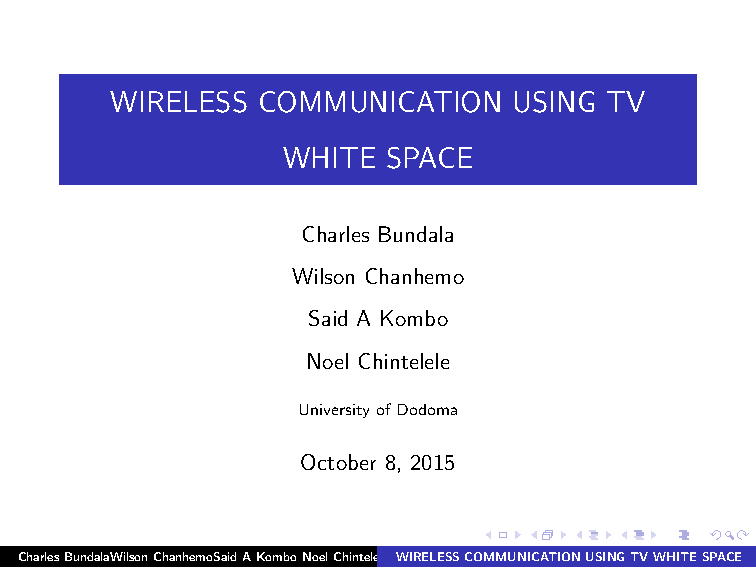
\includegraphics[width=1\linewidth]{best/TVWS}
\caption{1 TV white space}
\label{fig:TVWS}
\end{figure}
\end{frame}
\begin{frame}{MOTIVATION TO USE TV WS}
	\begin{itemize}
		\item{Driving force is due to spectrum shortage}
		\item {The huge growth of mobile data utilization has showed that current spectrum allocations for cellular or Wi-Fi networks are inadequate}
		\item {Drawback of strict regulation is that the spectrum utilization is not optimal. Depending on wireless system there can be substantial temporal and geographical differences how spectral resources are utilized}
		\item{The transition from analog TV transmissions to digital TV frees up large amounts of frequencies in VHF and UHF bands}
	\end{itemize}
\end{frame}
\begin{frame}{UNIQUE CHARACTERISTICS OF TVWS}
	\begin{itemize}
		\item {Most of the spectrum expected is already assigned to the primary user (licensee)}
		\item {Spectrum varies from region to region}
		\item {Dynamic Frequency Selection}
		\item {Avoidance of co-channel operation}
		\item {Adaptive Modulation/Coding}
		\item {Transmit Power control}
	\end{itemize}
\end{frame}
\begin{frame}{AVAILAIBLE STANDARDS:IEEE 802.22 WRAN}
	\begin{itemize}
		\item {Wireless Regional Area
			Networks (WRANs)}
		\item {Provide Wireless broadband access e.g to rural areas}
		\item{Topology: Point-to-multipoint and Master slave }
		\item {Entities: Base Station, Consumer Premise Equipment  (CPE)}
	\end{itemize}

	
\end{frame}
\begin{frame}{AVAILAIBLE STANDARDS\\IEEE 802.22 WRAN ...}
\begin{figure}
\centering
\includegraphics[width=0.6\linewidth]{best/WRAN}
\caption{}
\label{fig:WRAN}
\end{figure}	
	
\end{frame}
\begin{frame}{AVAILAIBLE STANDARDS\\IEEE 802.11af}
	\begin{itemize}
		\item {Wi-Fi extension to TVWS}
	\end{itemize}	
	\begin{figure}
\centering
\includegraphics[width=1\linewidth]{best/wifi-loc}
\caption{4: 802.11af}
\label{fig:wifi-loc}
\end{figure}

\end{frame}
\begin{frame}{AVAILAIBLE STANDARDS\\Others}
	\begin{itemize}
		\item {IEEE 802.16h WiMAX extension to TVWS}
		\item {IEEE 802.15.4m Extension of PAN standards to TVWS}
		\item{IEEE 802.19.1 Co-existence of several white space systems}
	\end{itemize}
	
\end{frame}
\begin{frame}{Sensing the TVWS}
	\begin{itemize}
		\item COGNITIVE RADIO
	    \item GEO-LOCATION DATABASES
	\end{itemize}	
\end{frame}
\begin{frame}{Sensing the TVWS\\COGNITIVE RADIO}
	\begin{itemize}
		\item {enable flexible, efficient and reliable spectrum use by adapting the radio’s operating characteristics to the real-time conditions of the environment}
	\end{itemize}
	\begin{figure}
\centering
\includegraphics[width=0.6\linewidth]{best/cognitive}
\caption{3 Geo-location Databases}
\label{fig:cognitive}
\end{figure}

\end{frame}	
\begin{frame}{Sensing the TVWS\\GEO-LOCATION DATABASES}
	\begin{itemize}
		\item {Collection of Databases indicating available TVWS channels}
	\end{itemize}
	\begin{figure}
\centering
\includegraphics[width=0.7\linewidth]{best/GEOLocation}
\caption{}
\label{fig:GEOLocation}
\end{figure}
\end{frame}
\begin{frame}{CURRENT RESEARCH CHALLENGES IN TVWS USAGE}
	\begin{itemize}
		\item {Spectrum Sharing and interference management}
		\item {Quality of white space channels}
		\item {Security challenge: Geo-location Databases are available in the public internet}
	\end{itemize}
\end{frame}

\end{document}
